The \ivfsystem{} was evaluated based on the implemented functions.
These functions are structured to the research workflow as described in \silvia{more explicit: figure? the introduction of section \ref{system-functionality}}. This workflow will now be referred to as the `process' of the system.
\silvia{?While evaluating found problems break down into fundamental flaws in the process and design flaws.}

\silvia{i think you put too much stress on "finding flaws" in this chapter. the purpose is to evaluate, not debug. the users will have opionions about what could be better, but these are not necessarily "flaws". Maybe some are design flaws, but this is something to conclude at the discussion session (4.2). I suggest you revise the terms you used to make the evaluation sound more neutral or even positive.}

For the purpose of the evaluation the \ivfsystem{} code was running on the local environment of a laptop.
No connection to the internet was necessary for testing, therefore performance issues were out of the question.
The used dataset was randomly generated (strings of letters), both because the \projectdata{} was not available yet and for privacy reasons \silvia{explain better or remove}.
Screenshots of the running gateway are shown in figures \ref{fig:standard-view-website} and \ref{fig:sunburst-view-zoom-website}.

\begin{figure}[!b]
	\centering
	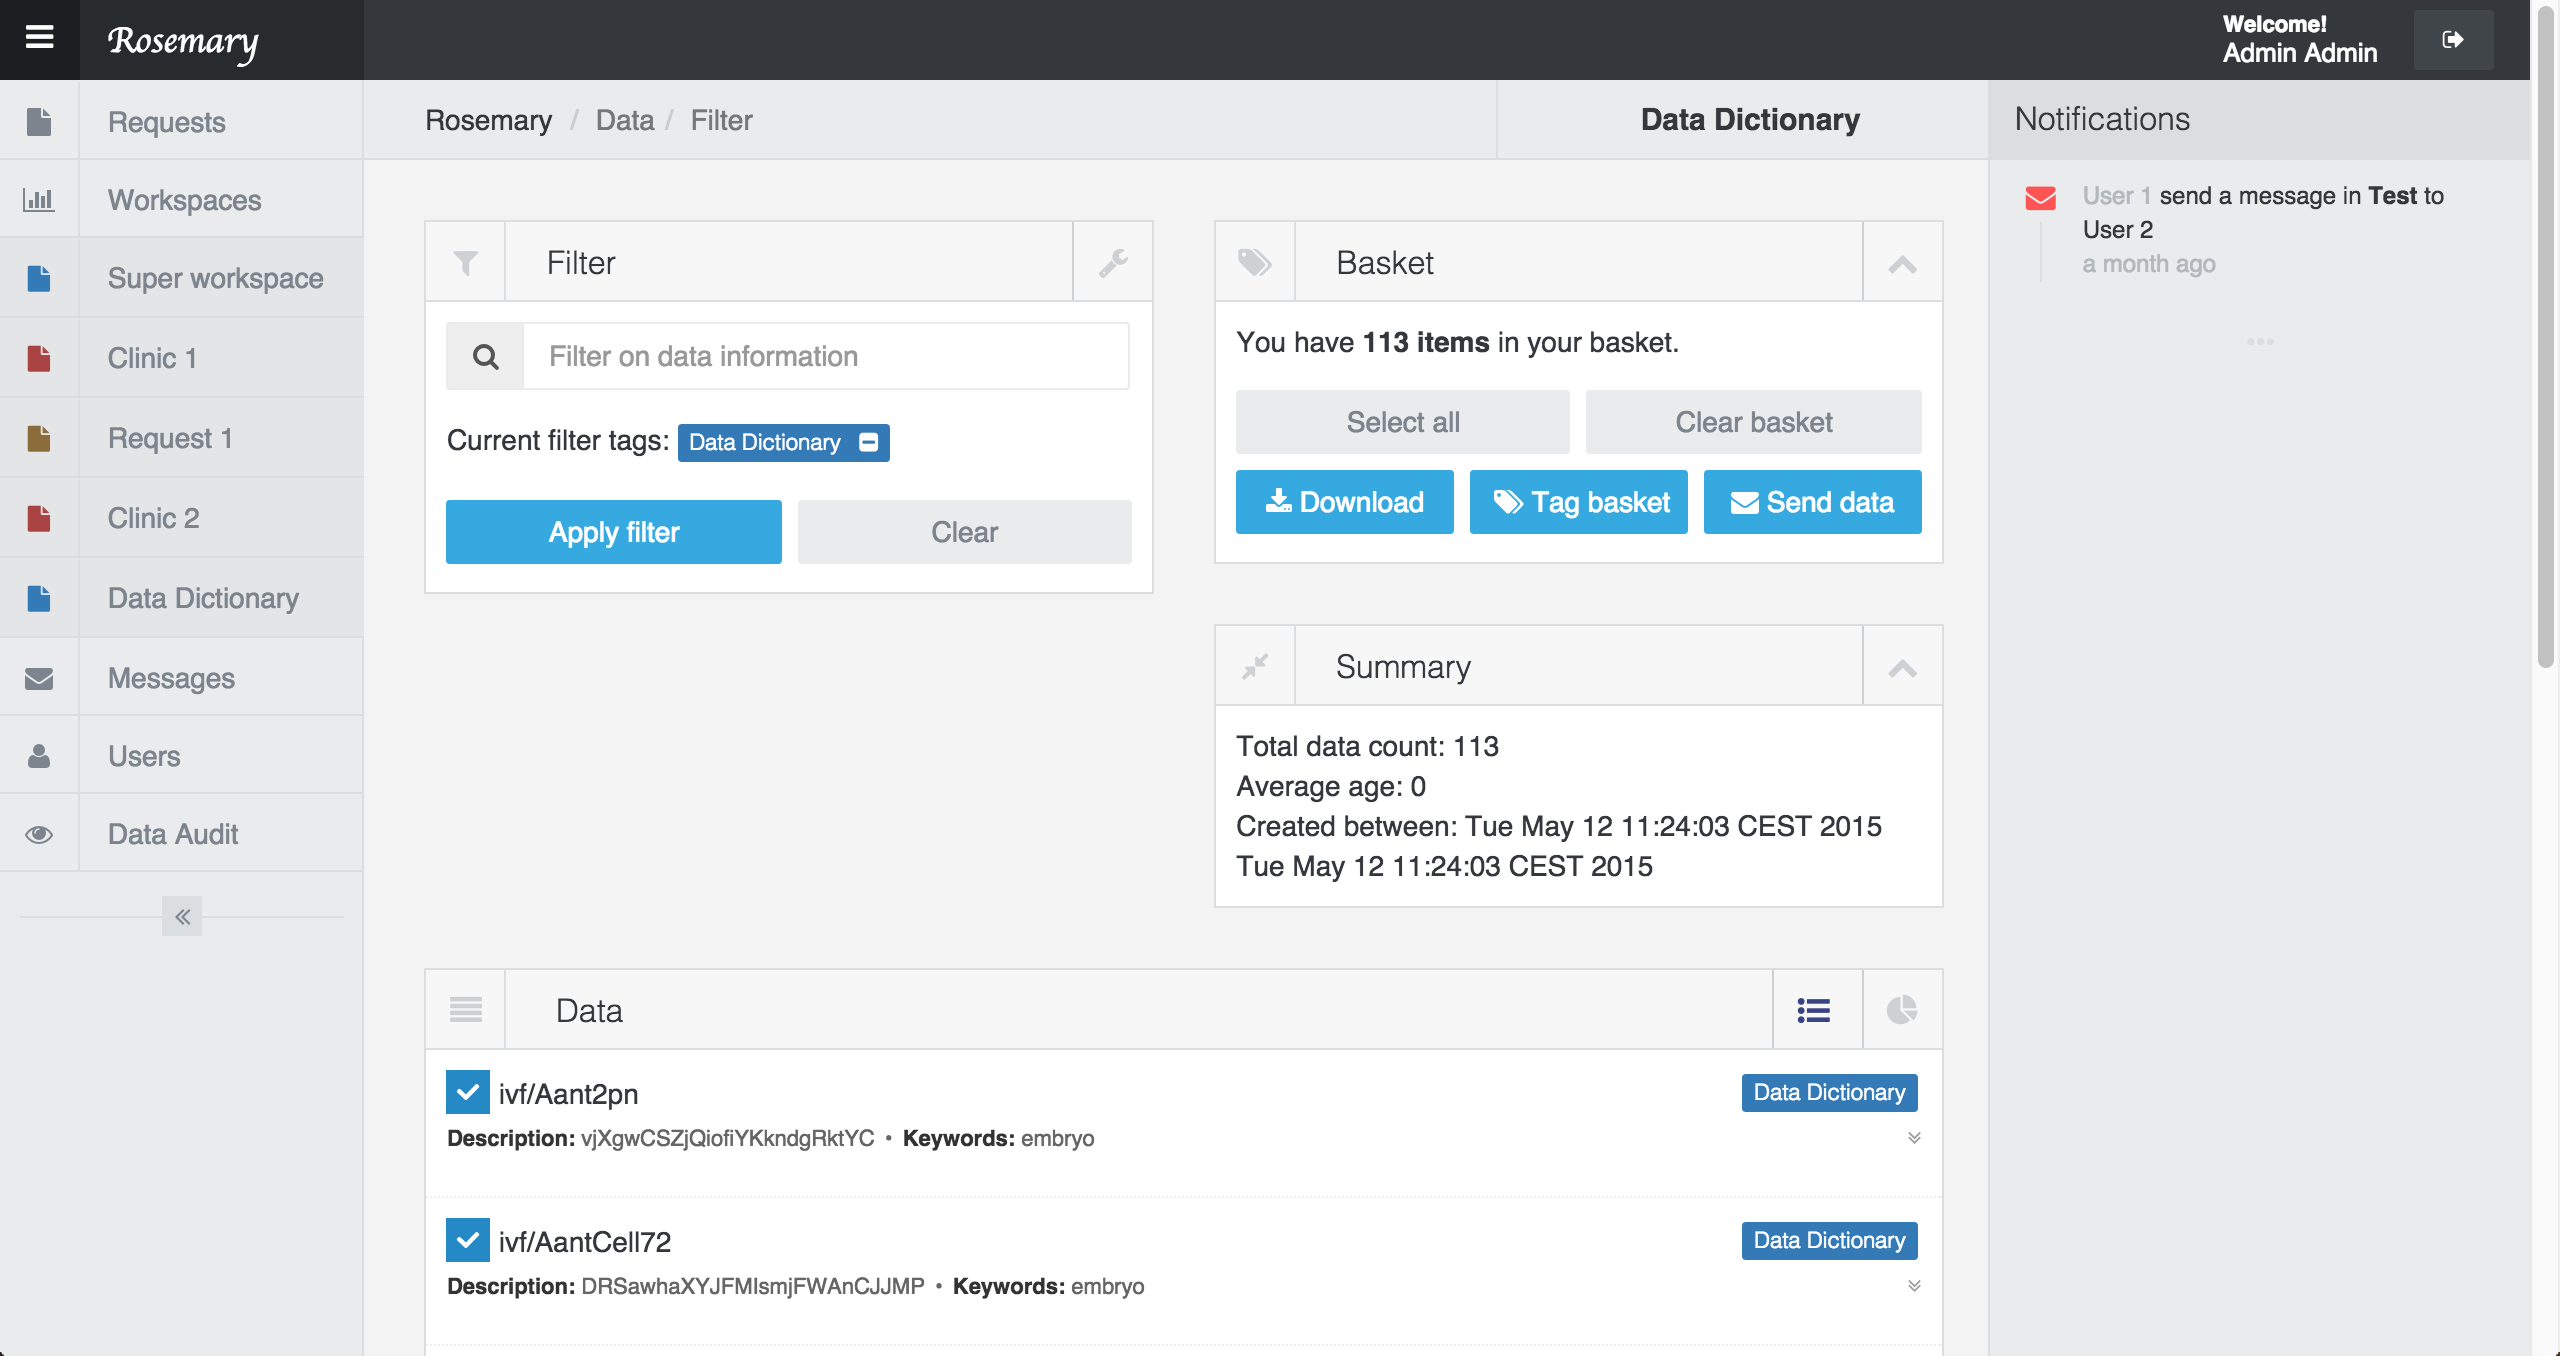
\includegraphics[width=1.0\linewidth]{images/standard-view}
	\caption{
		Running \ivfsystem{} data management view showing the standard display of the data (\ie{} summary on top and raw data at the bottom).
	}
	\label{fig:standard-view-website}
\end{figure}

\begin{figure}[ht]
	\centering
	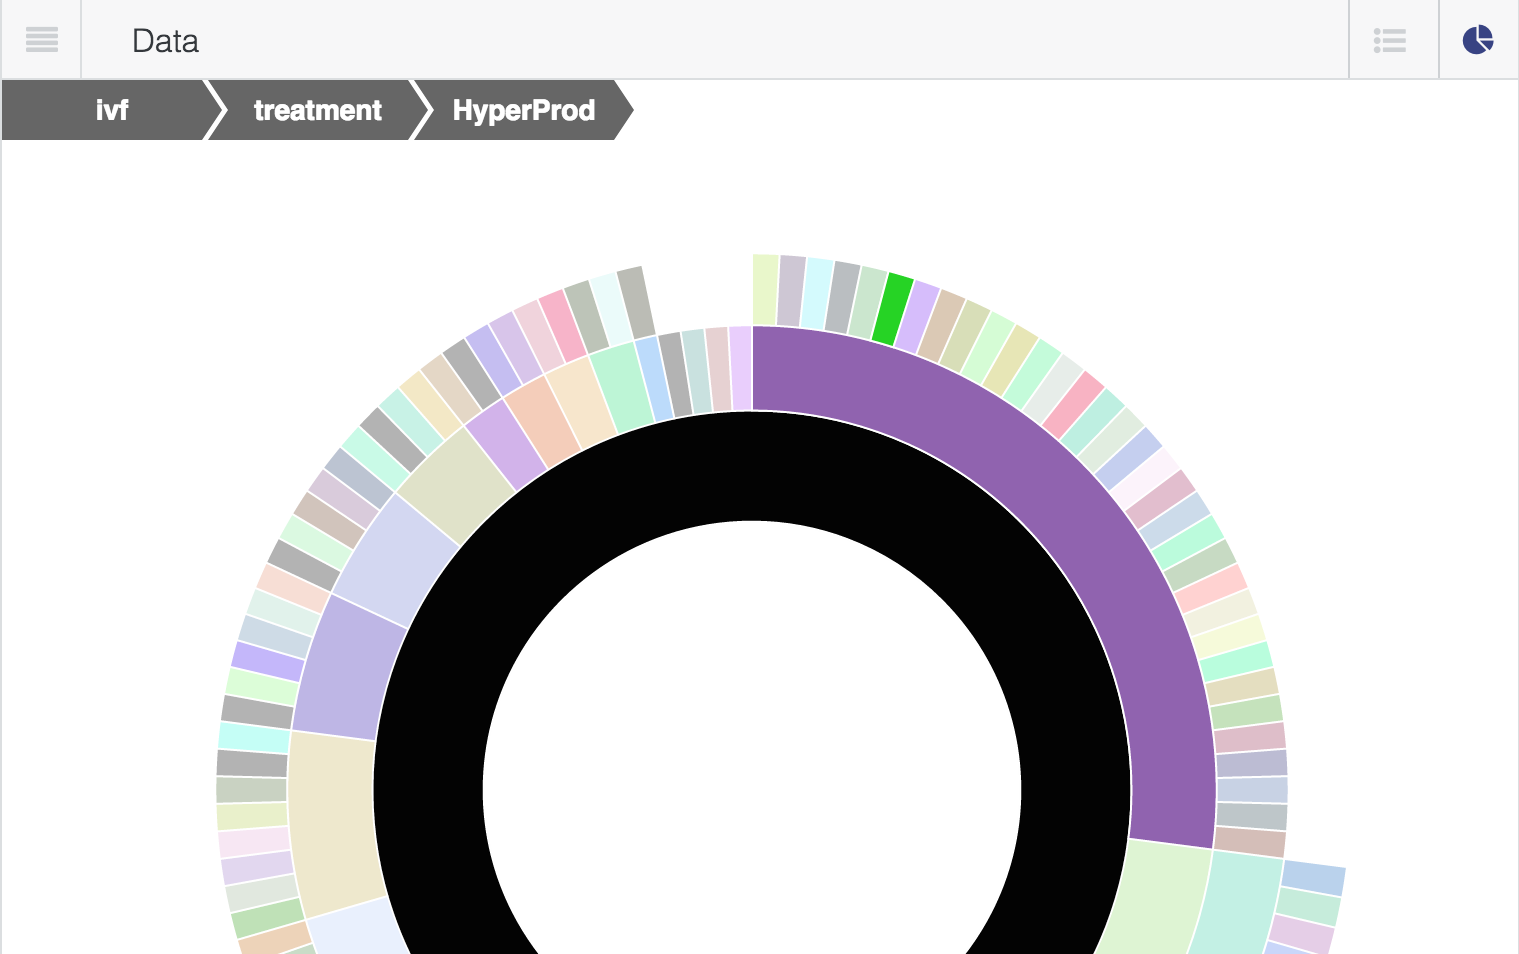
\includegraphics[width=0.7\linewidth]{images/sunburst-closeup}
	\caption{
		Running \ivfsystem{} data graph view showing the (sunburst) graph display of the data.
	}
	\label{fig:sunburst-view-zoom-website}
\end{figure}

All evaluations were done in an informal open-talk setting with no predefined questions.
First, the purpose of the meeting was explained in a few sentences.
Each user had to perform tasks using the prototype according to the assigned case: researcher, committee, administrator.
There were three testers, and some were assigned two cases because they fit in the field of experience of the respective user role.

\silvia{have you explained the concept of baskets, and presented the interface at all? the figure explains only the functions, and not the UI. If you had not, please say this explicitly here as a strategy - it seems you wanted the interface to be self-explanatory, which is very difficult to achieve.}
Tasks were described according to the system schema presented in figure \ref{fig:brainstorm-after}.
The interviewer only gave directions during the evaluation after the tester indicated that they did not know how to proceed.
If the tester struggled with a task the interviewer tried to encourage the tester to think aloud.
From this the process bottlenecks and design flaws of the system were identified.
Also, testers were asked to suggest design or process alternatives.

The  cases presented below are loose transcripts of the evaluation sessions.
After these the identified problems and possible improvements are summarised in section \ref{evaluation-summary}.

\section{User sessions transcripts}

\silvia{the nonsense data appears many times as "problem" - does it mean that the evaluation was not well prepared? has this hampered the conclusions? note that bad data is not design flaw - it is evaluation design flaw. Maybe to test the influence of this in the evaluation of the system you should put some sensible data and repeat one of the evaluations? there is no time for that, but you can comment on this in the discussion}

\silvia{the transcripts are messy, sorry. they are verbose and yet it is difficult to guess what you are talking about without seeing the system, or at least a proper description of the UI and how to perform each task (which is NOT included in chapter 3, and i agree it should not be.) \\
 So maybe one way to go around this would be to organize these transcripts like this: explain the task (high- level), how they should have done (not too much detail about clicking (unless you put some supporting screenshots, but this would make it very long), then explain how the users did it, including the comments and difficulties.}

\silvia{i also have the feeling that you are not specific enough in the text below when talking about tasks. you could define them at high-level ('approve request', consult colleague, ??) or a lower level (find list of requests, identify pending ones, find information about pending in order to decide, approve. I think the evaluation is different for each of the micro-tasks. the system could be good in general for finding things on the UI, but not for selecting things, for example. By being more detailed about the various tasks it will also be possible to draw conclusions across the user roles, as the system uses the same mechanisms that might have revealed less intuitive than expected.}

\paragraph{Researcher Role}
From all the cases this is arguably the largest as it has the most extensive (implemented) functions.
%Therefore, all the testers performed the researcher tasks to find more flaws or give more support to flaws found with both testers.
The tasks that had to be performed were: search the data dictionary for headers, use these data headers to compose and submit a request, download the requested data.

Finding the data dictionary was not a big problem for the testers.
The next step is filtering, which is relatively easy as the input is text based and the search itself is fuzzy.
Dictionary items can be sought for based on name, description, and keywords.
Because in the prototype the descriptions are nonsense, it was difficult to find the wanted data headers.
Two of the testers did not notice that the search is instantaneous (like google search).
This resulted in pressing 'enter' and clicking the `apply filter' button multiple times before noticing that the data had already changed at the bottom of the screen.
One of the testers prefers to search the data off-line, \ie{} print the fields and later select the wanted items in the interface.

The difficulties in using the filter function, plus the nonsense data, made it rather hard for the testers to find the desired headers. 
\silvia{explain task first, then the impressions from the users: They were asked to select a couple of random headers to start a request with.}
Selection was straightforward but the testers did not notice that selected items were added to the basket. \silvia{is this repeated?}
Therefore, two asked `how do I keep this selection when I start searching again?'.
This also resulted in two of the testers using the `select all' function on the basket. 
Clicking this will make a selection of \emph{all} the items in the workspace, basically overwriting the previous basket and losing all the progress.

To proceed in the task of making a request the testers looked for a button on the basket.
However, the buttons are specific to a 'raw data view' and do not make sense in a 'dictionary view' of the system.
The testers needed to be explained that the basket is kept in the back of the system and can be used over multiple views.
\silvia{reformulate: Clicking the request button at the top left of the screen is the correct action, then selecting `new request' results in a form with the basket attached showing which items were selected.}

Data download is straightforward. This is done by going to the correct workspace from the menu on the left, selecting the wanted items (or 'select all'), and clicking the `download' button.
No problems were found here, however one of the testers noted that in principle \emph{all} data will be downloaded every time. \silvia{is this a problem or a good feature?}

\paragraph{Committee Member Role}
The committee tasks are the shortest, as the list only contains the request approval function. 
It breaks down into finding the requests which are open for approval, evaluating them against already approved requests, and voting.
Viewing requests that are ready for approval is done by selecting the `request' button from the left menu.
Now a list is shown of all these requests and the data that is necessary for making the decision.
Approval is given (or not) by selecting a approve or disprove button, a vote remains open for change until all committee members have casted their vote.
The actual vote is shown both with a symbol (V/X) as with a colour (green/red).

\silvia{ok, so this part is already in good shape, describing first what the user should have done. now you need to add one sentence saying how the user did it }

\silvia{is this a new task? then it is not only approval!}
Communication functions are built into the view.  
Clicking on one of the requests redirects to `new message', the user can create a message which (upon hitting send) is automatically send to all committee members.
There was a suggestion to add a comments thread to the request itself, instead of the separate message construction.
Furthermore, \silvia{?the redirect} was confusing for the tester as the expectation was that it would lead to more information on the request, even though all the available information was already shown. \silvia{so this means that they need more information to decide - what more do they need? is the info in the system or should the data model be extended?}

\paragraph{Data administrator Role}
Lastly, the data administrator performed the user management functions.
%The user overview is not complex in 
A list of users is shown, and each item contains buttons to perform the following actions: make committee member, make active, approve.
\silvia{i cant recall in chapt 3 to have read what are the transitions of user role. for example, can a committee member also have researcher role? or does this need another account, or is this forbidden by policy?}
This was clear and would be easy to use in a real-life scenario.
However, the tester noticeed that there are some process flaws.
If one of the users of the system changes institutions, most of the time the data manager is not informed, this is left to the P.I.s.
Therefore the system should contain support functions for non-administrators to view the list of users and communicating with the data manager about what actions should be taken.
\silvia{need to better explain this. why is the organization of the user important? for all users or for a particular role? it was not mentioned before. Also, who are the PIs? afaik there is no role for PI in this system. we have researchers, committee and data manager. does any of this map to what you call PI here?}